

\section{SPL Architecture with SMarty}
\label{sec:spl_smarty}

The SPL methodology differs from the development of singular software by the postponement of project decisions. The features are included in the software by convenience and the need of stakeholders. In the proposed SPL, the variabilities are concentrate in the \textit{business layer} features \cite{marcolinoarcht2017}. 

The integration of the teaching of programming domain, mobile platform and teaching and learning processes presents several features. The most of them need to be combined to provide a richer learning environment, allowing the achievement of the educational objective. The several features considered in the proposed SPL come from the analysis of 81 applications and software systems in the programming domain \footnote{\url{goo.gl/EvzUpB}}. Consequently, the catalog was represented in a feature model, depicting the relation among features, variabilities, variation points, variants and their constraints. As previously mentioned, SMarty was selected to represent this in UML diagrams. 



Among the \textit{domain design} sub-processes, the \textit{logical view} is represented through the feature model \cite{LindenSchmidRommes07}. The \textit{development view} can adopt the package diagram, component and class diagram. Figure \ref{fig:comp} shows the component model of the SPL.  



\subsection{Component Architecture}

The component diagram depicts how components are wired together to form larger components or software systems. They are used to illustrate the structure of arbitrarily complex systems\cite{Pressman:2015}. The SPL representation has four layers: \textit{client apps}, \textit{API gateway}, \textit{microservices} and \textit{repositories}.

\textit{Client Apps layer:} this layer shows the apps, platforms, websites, services or any potential consumer of the microservices. The main clients considered in the research are \textit{mobile apps}, followed by \textit{websites}. These clients have just the view and controller of the application. All the business logic is inserted in the microservices. However, they are the main way to wire together all the desired features by the tenant/user, previously selected in the \textit{application mechanism}. Additionally, all the clients are considered optional variabilities, since they may or not be part of the SPL. 

\begin{figure*}[!h]
    \centering
    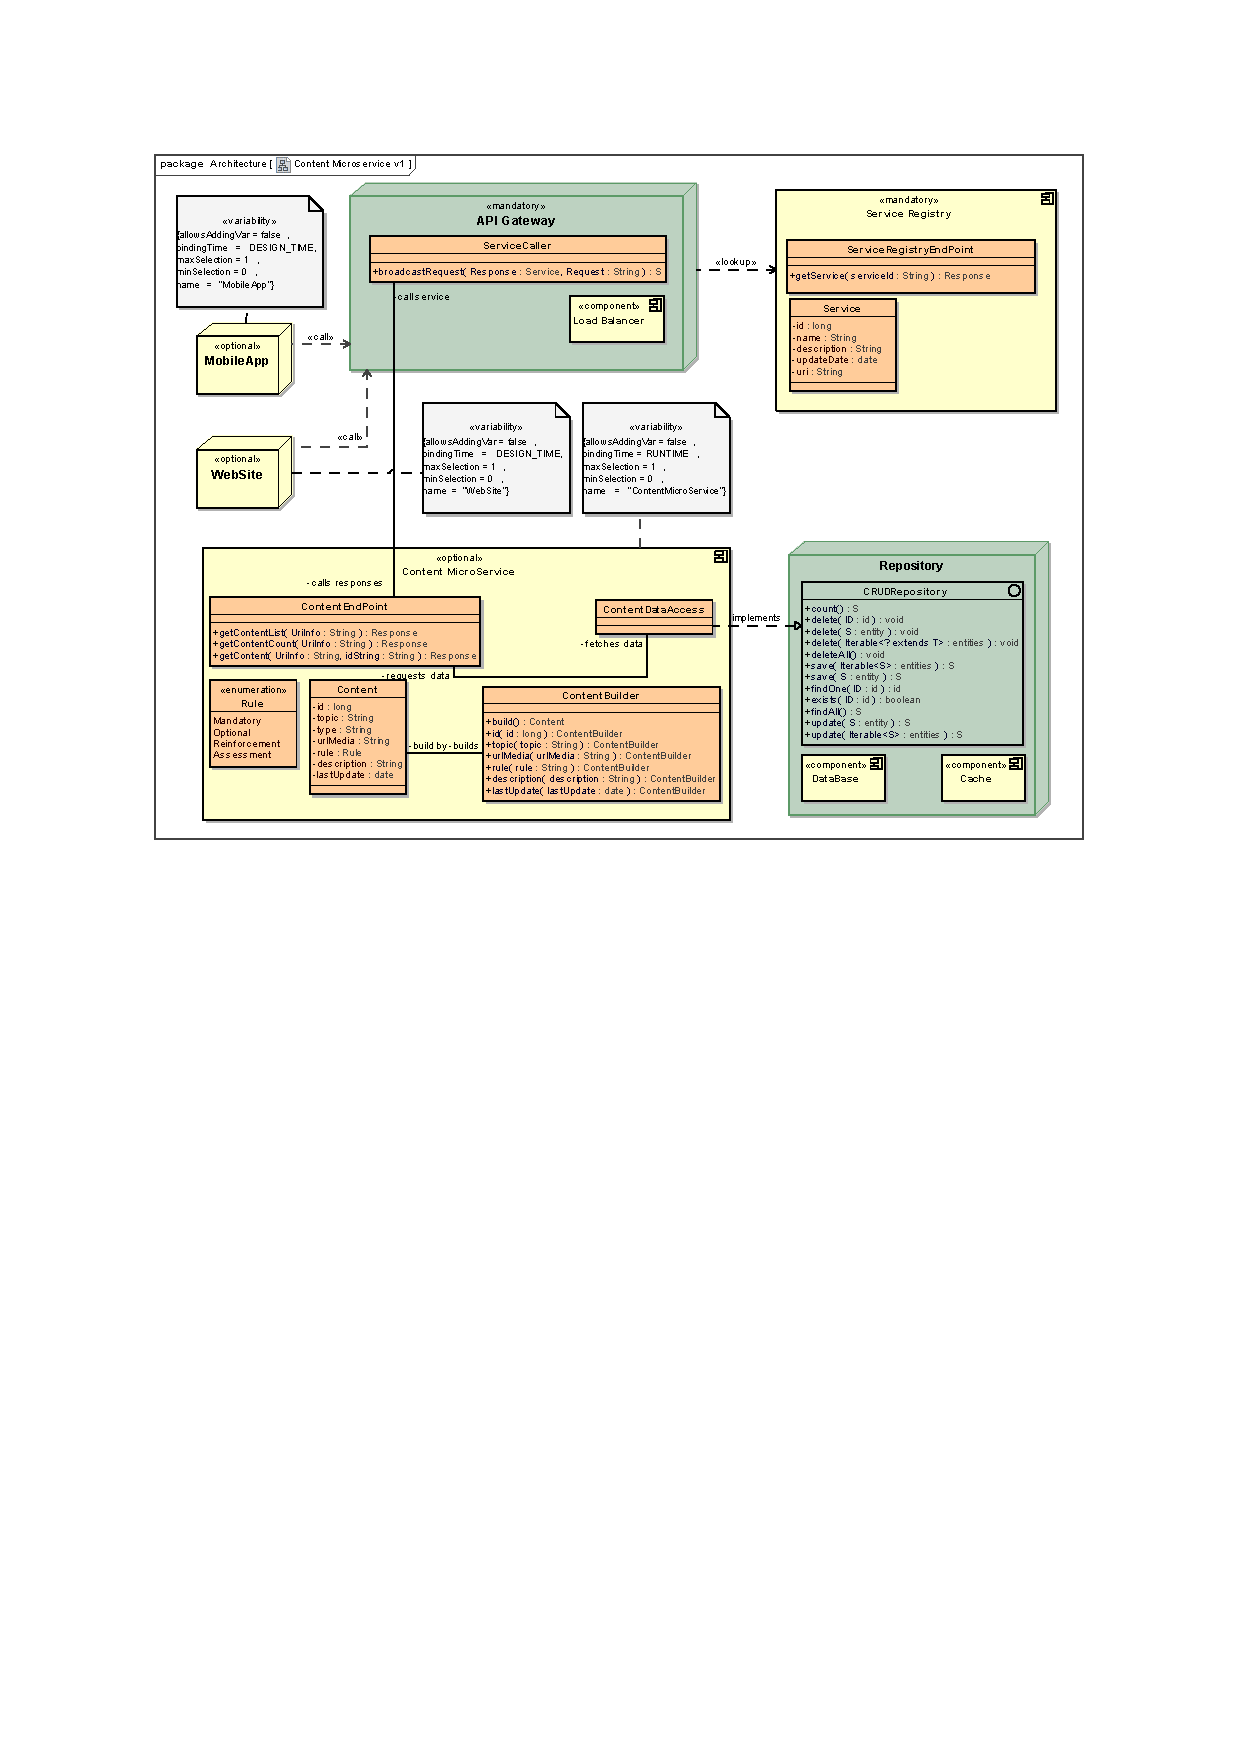
\includegraphics[scale=1.00]{content.pdf}
    \caption{M-learning SPL Content Microservice Class Diagram.}
    \label{fig:class}
\end{figure*}



In the representation, the clients are tagged as $\ll$optional$\gg$ and each one has a UML comment which depicts additional information about them. Those variabilities are solved in design time. Each instance of client calls the \textit{API Gateway} node from the next layer.





\textit{API Gateway:} this layer identifies the available microservices registered in a data base through the mandatory \textit{service registry} component. The \textit{API Gateway} node, also mandatory, looks up for the microservice requested by the client in the \textit{service layer}. If the microservice is found, the requisition is broadcast for the respectively microservice in the next layer. Additionally, the \textit{load balancer} observes the behavior and quantity of requests from the clients, balancing the load of data traffic and ensuring that all the requests will be answered, controlling them in a row. This component is also responsible to increase the server resources; in other words, it provides the elasticity of the cloud resources \cite{Pressman:2015, Newman:2015:BM:2904388}.




\textit{Microservices layer:} this layer encompass all the microservices, although each one can stay hosted in different servers. The microservices has specific functionality, from non-functional to functional ones and each represents the features depicts in the feature model. They are instances of each selected feature in the \textit{application mechanism}. The model presents four samples of services. Everyone has a component which express the type of supported protocol and, based on this protocol, each one receives requests directed by the \textit{API Gateway}. Still in this layer, each microservice is tagged as optional variability, but following the feature model, some of them will be represented as exclusive ($\ll$alternative\_XO$\gg$) or be mutually exclusive among the other microservices selected. For instance, educational activities can be available following a fixed order or be performed by convenience, therefore, these two features of the availability of educational activities follow the SPL mutually exclusive constraint. On the other hand, there are features that require others, such as the learning monitoring and performance, that needs feedback features to support both teachers and students.

Other behavior on the microservice layer is the possibility for the microservices to do calls among them, when it depends on the process of another microservices, removing the needs of processing from the client. These calls among the microservices is also performed by the API gateway.




\textit{Repositories Layer:} in this layer all repository structure is presented. They can be in different servers and, in some cases, they are not mandatory for some services. The repository is responsible for the management of the persistence process, providing interfaces in DAO model, if convenient, for enabling the access of the data in their registered data base. They also coordinate the cache usage.




\subsection{Architecture Class Diagram}





The next architecture artifact from the SPLE framework is the class diagram (Figure \ref{fig:class}). For this representation, as each microservice represents a feature, or a small set of them, the class diagram was divided in one representation for each existing artifact. This decision was made based on some issues, particularly: (i) the reduced number of developers, (ii) the reduced time for the development of each feature before its development, (iii) the facility to manage each diagram of the architecture as an artifact from the SPL core asset; and (iv) the the extreme programming (XP) agile process \cite{Beck:2004:EPE:1076267} with the test driven development (TDD) \cite{Fraser:2003:TDD:1763875.1763973} adopted for the conduction of domain realization and domain testing SPLE sub-processes (an investigation about this adoption will be conducted in order to provide evidences of the possible benefits in SPL context) .




%As consequence of the reduced number of developers and the big number of features to be developed, a questionnaire has been applied with programming teachers to identify the priority of the features.  Based on the results, a set of candidate features was selected in the conduction in the first iteration of the domain realization and testing sub-processes. Furthermore, based on the number of developers, the adoption of an agile methodology was included in the SPL project, the extreme programming (XP) agile process \cite{Beck:2004:EPE:1076267} with the test driven development (TDD) \cite{Fraser:2003:TDD:1763875.1763973}.




%Extreme programming process is iterative and incremental. It is an agile process because it emphasizes the communication and feedback among the project team. However, the main motivation to its adoption was the frequent iterations and its short releases, which eliminates defects earlier, reducing costs and meeting the objective in the adoption of microservices: the fast development of features, the fast availability for the customer and the concentration of efforts in short releases.



%\begin{figure*}[!ht]
%    \centering
%    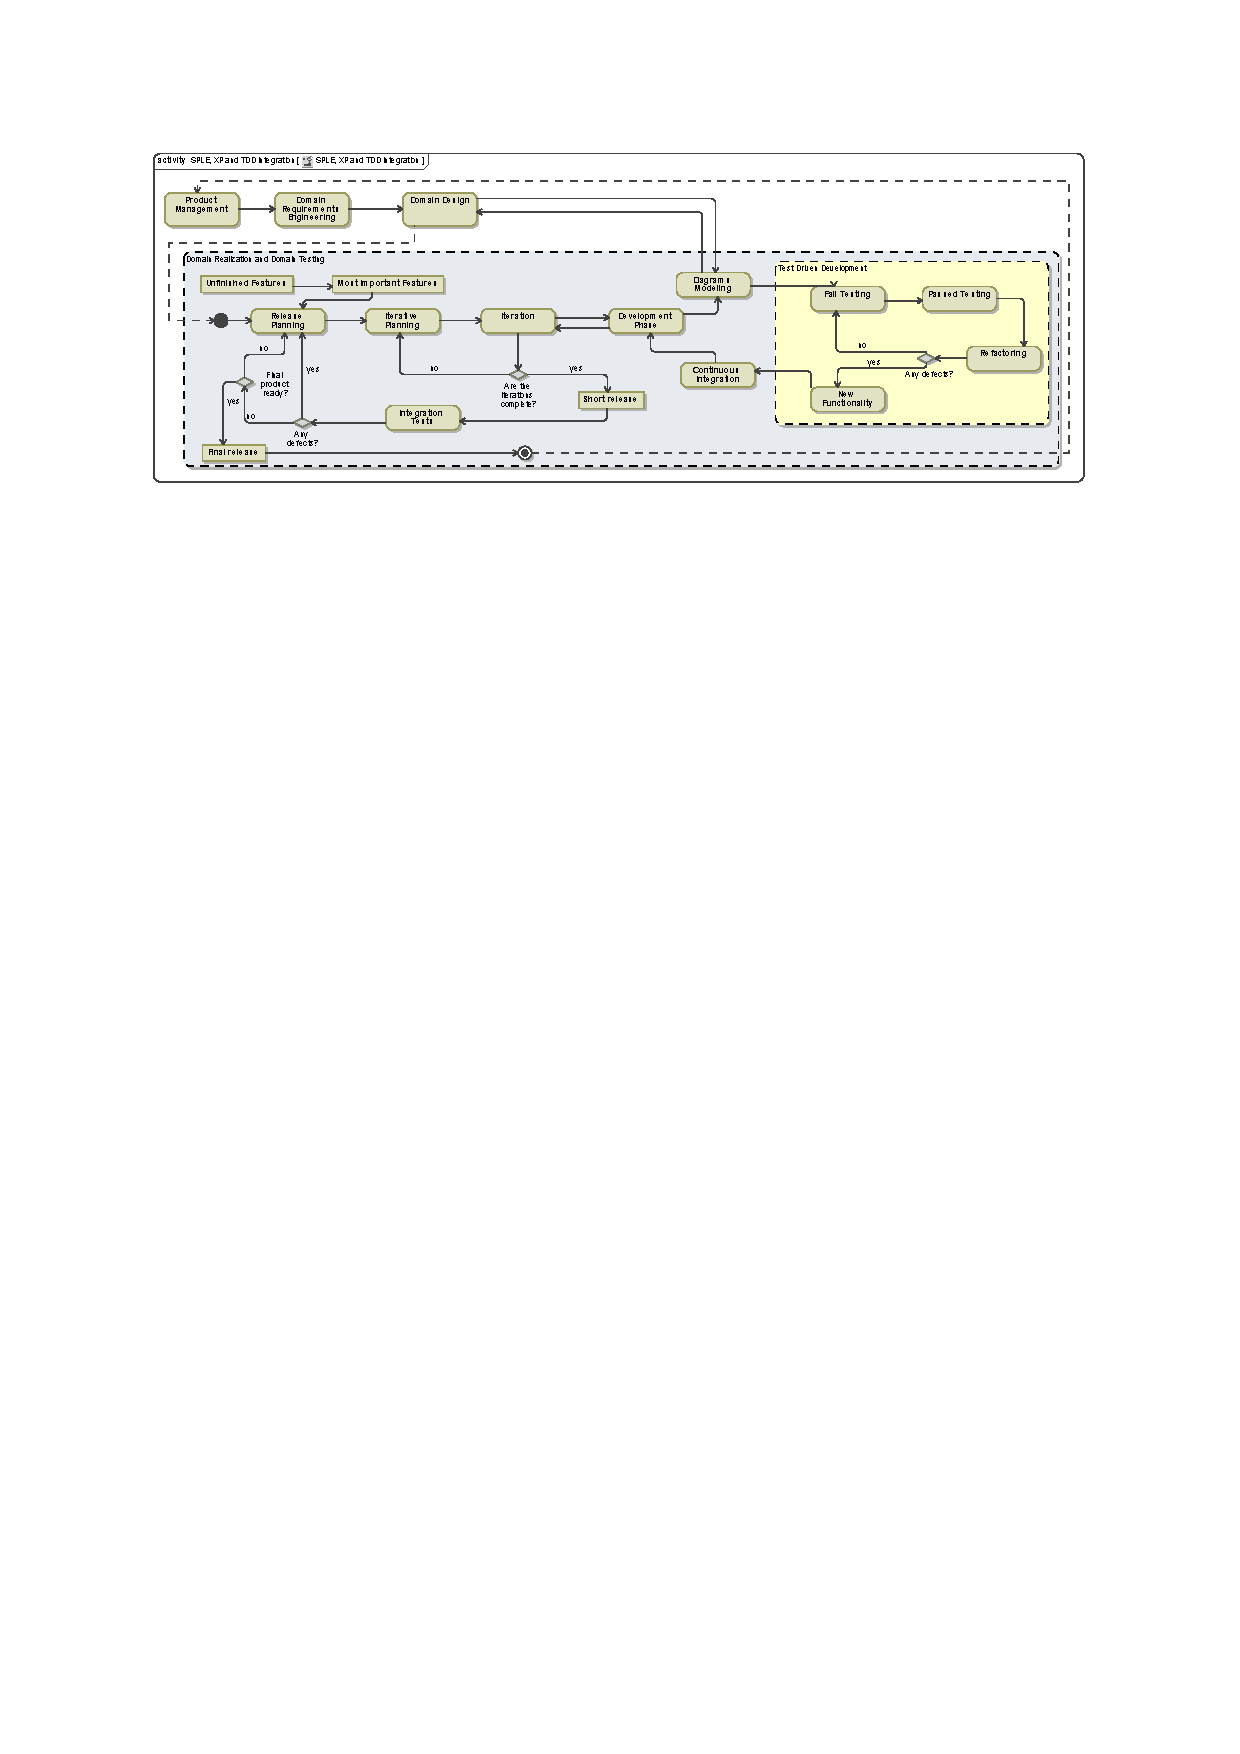
\includegraphics[scale=1.11]{activity.pdf}
%    \caption{Activity Diagram with the Integration of SPLE, XP and TDD.}
 %   \label{fig:activity}
%\end{figure*}


%In this perspective, to integrate and to agile the domain test realization, TDD was adopted together with XP. Such development technique has its base on the repetition of short cycles. Each development of a new functionality starts from the definition of a test. This test must fail because it is wrote before the functionality be implemented; if it fails, the proposed functionality or improvement is obvious. To write a test, the developers may understand the specifications and requirements of the functionality. It can be done through uses cases or use stories that cover the requirements and the conditional exceptions. In the context of the line, the requirements catalog with the feature model and its constraints were considered. This is the main difference from the process of writing unit tests after the code is ready. It keeps the focus of the development in the requirements before the coding, which is a subtle but important difference.

%After the definition of the test that must failed, the next phase is to check if the new test does not bring errors. In other words, this phase tests its own test. Next, the test must failed by the expected reason: the functionality has not been developed yet. In the next phase the code which must pass in the test is developed. 

%The developed code can be wrote presenting some problems or did no pass in a elegant way, since the next step will be improved it. The aim is to write a code that pass in the test. If the developed code passes in all the tests, it means that all the requirements were considered in the code, starting the final phase of the TDD: the coding refactoring. In this phase, the code is improved, removing redundant code and verifying if it still passes in the tests cases previously checked. In this phase, the modeling of the class diagram of such functionality is performed and the cycle is started again. With the development of a new functionality, the continuous integrity has a fundamental role to provide reversible points, once a union of functionalities could generate errors, when integrated.

%After the TDD cycle, the XP cycle continues. The functionality released is analyzed in a integration test and, if passed, the release can generate the expected product or be stored in the core asset to be integrated after, with other functionality to be developed.


%Figure \ref{fig:activity} depicts an activity diagram that summarizes the integration of the XP agile process and TDD technique tasks with SPLE framework sub-processes.


Figure \ref{fig:class} shows the content feature microservice represented in a class diagram. The diagram considers two instances of clients: an \textit{MobileApp} and a \textit{WebSite}. Both calls the content \textit{API Gateway} which look up in the \textit{Service Registry} to identify if the requisition for such microservice can be answered. For this, the respective called microservice need to be register on the queried data base and be identified with the support of a \textit{repository}. With the identified service, the \textit{API Gateway} can localize the service through its \textit{uri}, executing the request that comes from the customer and returning to it the retrieved content data being presented in their app interface through the controller of content and its communication with the presentation logic layer.

Three variabilities are represented in the class diagram. The two clients, where both are solved in design time; and the content microservice, that is solved in runtime. The content microservice is considered a variability because some learning applications can be developed only to provide activities for the students, not being mandatory for every application. The difference among the binding time of the variabilities is related with the type of variability. The clients need to have its presentation and business logic layers developed before, since they will consume the available microservices accordingly to the permission of features selected for users on the \textit{application generation mechanism}. The availability of the microservices, in turn, will occur in runtime. All microservices will be available for the client applications, although only the ones that the user logged in the application have permission or were selected to their users will be visible and can be used.




\subsection{Lessons Learned}

Based on the tasks and decisions made on this research, the two main lessons learned were:

\begin{itemize}
\item Evaluate the requirements catalog and after, the first conceptual model architecture without a integration of both could be resulted in future problems in development phase. This was made based on the order of research phases and this threat was mitigate based on the practitioners analysis.
\item Microservices improve the reuse and, in some cases, can be adopted in other software programs independently of the domain. Additionally, the reduced size of functionalities expressed on them enables the creation of a greater number of configurations of application. In this perspective, other microservices can be easier integrated to our solution and even, our microservices can be reused in other contexts. However, the evolution of the line will need more attention, since the communication among these microservices requires more efforts and tests to guarantee that they will work properly.



\end{itemize}


%It is also important to highlight that the integration of the XP process and TDD technique in the SPLE framework needs to be better investigated in order to provide evidences of the possible benefits when considered to create an infrastructure for the development of mobile learning applications for the teaching of programming. This is a topic for future research.

